\subsubsection{类的基本概念}

类是\textbf{面向对象}(OB,Object-Oriented)最基本的概念,也是C++区别于C语言的重要特征。
面向对象编程的基本思想是抽象出对象,将对象作为程序的基本单元,通过消息传递来进行通信和协作。
对象是类的实例,具有状态和行为,状态存储在对象的数据成员中,行为由对象的方法实现。
对象通过消息传递进行通信,对象之间可以互相发送消息,并处理消息。
面向对象编程的优点是代码的可重用性、可扩展性和可维护性都得到了提高。

在C++中,类是一种抽象数据类型,它定义了对象的行为和状态,并提供了对这些数据的访问接口。
类可以包含数据成员、成员函数、构造函数、析构函数等,这些成员构成了类的接口。
类可以派生出新的类,从而实现代码的重用和扩展。

\begin{tcode}
class ClassName{        //类名
    public:             //修饰限定符public
        ClassName();    //构造函数
        ~ClassName();   //析构函数
        void memberFunction();  //成员函数
    private:                    //修饰限定符private
        int dataMember;         //数据成员
        void privateFunction(); //私有成员函数
}    

\end{tcode}

\begin{enumerate}
    \item \textbf{构造函数和析构函数}:类的构造和析构过程,它们负责对象的初始化和释放,其特点是其函数名与类名相同,没有返回值。
    \item \textbf{成员函数}:实现类的行为,它们实现了类的功能。
    \item \textbf{数据成员}:存储类的数据信息。
\end{enumerate}
\begin{center}

    \begin{tabular}{cc}
        \hline
        修饰限定符 & 作用 \\
        \hline
        private & 只能被类的成员函数使用或调用 \\
        public & 可以被类外的其他函数或派生类中函数调用 \\
        protected & 只能被类的成员函数和派生类使用或调用 \\ 
        \hline
        
    \end{tabular}
\end{center}

% 类可以派生出新的类,派生类可以继承基类的所有成员,并可以添加新的成员。
% 派生类可以重写基类中的成员函数,从而实现新的功能。
% 派生类可以重载基类中的运算符,从而实现新的运算。

面向对象编程的实现方式有多种,包括面向过程、基于消息的、基于事件的、面向对象设计模式等。
面向过程的实现方式是将数据和函数分离,通过函数调用来实现对象之间的通信。
基于消息的实现方式是通过消息传递来实现对象之间的通信,消息可以是函数调用、事件、数据等。
基于事件的实现方式是通过事件驱动模型来实现对象之间的通信,事件可以是用户操作、时间事件、状态变化等。

\subsubsection{静态和友元}

静态成员是指在类外部定义的变量和函数,它属于整个类,而不是类的对象。
静态成员可以\textbf{被类的所有对象}共享,因此可以实现一些全局变量的功能。
静态成员的声明和定义都在类的外部,因此在类的声明中不需要加$static$关键字。

需要特别注意的是,静态变量的定义必须在实例化之前。静态成员的生命周期和整个程序的生命周期是相同的,因此静态成员的构造函数和析构函数只会被调用一次。
\begin{enumerate}
    \item 友元函数:友元函数可以访问类的私有成员,但不能调用类的私有成员函数。
    \item 静态成员:静态成员可以被类的所有对象共享,因此可以实现一些全局变量的功能。
    \item 静态变量:静态变量的定义必须在实例化之前。静态成员的生命周期和整个程序的生命周期是相同的,因此静态成员的构造函数和析构函数只会被调用一次。
\end{enumerate}

\begin{tcode}
class ClassName {
    public:
        ClassName() = default;
    
        ~ClassName() = default;
    
        static void memberFunction();   //成员函数
        static int dataMember;          //数据成员
        friend void FriendFunction(int a, int b);//友元函数定义
    private:                            //修饰限定符private
        static void privateFunction();  //私有成员函数
};
        
void FriendFunction(int a, int b){ //友元函数实现时,不可以添加类的作用域
    std::cout << "你调用了友元函数";
}
        
int ClassName::dataMember = 10; //静态变量只能在类的实例化之前定义
        
int main(int argc, char *argv[]) {
    ClassName obj1, obj2;
    cout << obj1.dataMember << endl;
    cout << obj2.dataMember;
        
    return 0;
}

\end{tcode}

有时,我们希望某个函数可以访问类的私有成员,但又不希望它成为类的成员函数。
这时,我们可以将函数声明为友元函数,并在类的声明中加上$friend$关键字。
友元函数可以访问类的私有成员,但不能调用类的私有成员函数。

\textbf{需要注意的是,不属于类,它破坏了类的封装性,因此不建议使用!}

\subsubsection{函数重载}
\textbf{函数重载(overload)}是指在同一个作用域中,存在多个同名函数,但它们的参数个数或参数类型不同。
函数重载的作用是为了使程序更加灵活,提高代码的可读性和可维护性。

在C++中,函数重载的规则是:
\begin{enumerate}
    \item 函数名相同;
    \item 参数个数不同;
    \item 参数类型不同。
\end{enumerate}

\begin{tcode}
class ClassName {
public:
    ClassName() = default;

    ~ClassName() = default;

    int CalSum(int a,int b){
        return a+b;
    }

    double CalSum(double a,double b){
        return a+b;
    }
};

int main(int argc, char *argv[]) {
    ClassName obj;
    cout << obj.CalSum(1,2) << endl;
    cout <<  obj.CalSum(1.5,2.5);

    return 0;
}
\end{tcode}

在上例中,CalSum函数的两个版本都可以接受两个参数,但它们的返回值和参数类型不同。
因此,我们可以实现两个函数的重载,使得程序更加灵活。在执行函数时,编译器会根据函数的调用情况,自动选择最匹配的函数版本。

\textbf{构造函数的类型:}

\begin{enumerate}
    \item 默认构造:默认构造函数是指没有参数的构造函数,它会创建一个对象,并对其进行初始化。
    \item 含参构造:含参构造函数是指有参数的构造函数,可以根据参数的值对对象进行初始化。
    \item 拷贝构造:拷贝构造函数是指将一个对象拷贝到另一个对象时,会调用拷贝构造函数。
\end{enumerate}

\begin{tcode}
#include<iostream>
#include<string>
class ClassName {
public:
    ClassName():member(1) //初始化列表
    {std::cout << "你调用了默认构造函数" << std::endl;}
    ClassName(std::string& str) 
    {std::cout << "你调用了含参构造函数,参数是" << str << std::endl;member=2;}
    ClassName(ClassName &obj) //这里必须是引用传参,思考一下为什么
    {std::cout << "你调用了拷贝构造函数" << std::endl;
    this->member = obj.member;}
    ~ClassName() = default;

    int member;
};

int main(int argc, char *argv[]) {
    ClassName obj1;
    std::string str = "Hello World";
    ClassName obj2(str);
    obj1.member = 10;
    ClassName obj3(obj1);

    std::cout << "obj1:" << obj1.member << std::endl;
    std::cout << "obj2:" << obj2.member << std::endl;
    std::cout << "obj3:" << obj3.member << std::endl;

    return 0;
}
\end{tcode}
有一些tips可以快速设置构造函数
\begin{tcode}
ClassName() = default;              //默认构造函数,使用默认的方式
ClassName(ClassName& obj) = delete; //禁止拷贝构造,单例实现对象
\end{tcode}
\textbf{运算符重载:}

在C++中,类提供了一个接口,可以将运算符进行重载,从而实现对类更加灵活的操作。
运算符重载的语法如下:

\begin{tcode}
[返回值] operator [操作符] ([参数列表]) {
    //操作符的实现
}
\end{tcode}

示例:

\begin{tcode}
class ClassName {
    public:
        ClassName():a(1),b(2) {}
    
        ClassName& operator+(ClassName& obj){//重载加法运算符
            this->b += obj.b;   //this指针,指向自己
            this->a += obj.a;
            std::cout << "这里执行过了" << std::endl;
            return *this;   //*this表示当前对象的引用
        }
     
        //重载流插入运算符,思考一下为什么是这样写?
        friend std::ostream& operator<<(std::ostream& out, ClassName& obj);
    
        int a;
        int b;
    };
    
    std::ostream& operator<<(std::ostream& out, ClassName& obj){
        out << "a:" << obj.a << " b:" << obj.b << std::endl;
        return out;
    }
    
    int main(int argc, char *argv[]) {
        ClassName obj1;
        ClassName res = obj1 + obj1;
        std::cout << res;
    
        return 0;
    }
\end{tcode}

\textbf{$this$指针}是一个隐指针,指向这个类本身。
在类的成员函数中,$this$指针可以用来访问类的成员变量和成员函数。
在类的构造函数中,$this$指针可以用来初始化类的成员变量。
一般情况下,$this$指针可以不写,编译器会自动生成。但是有些情况,处于项目代码可读性的目的,会写显性的$this$指针。
此外,类中成员函数的第一个参数必须是$this$指针,表示当前对象的引用。这也是类的成员函数的调用方式。在后面我们会详细解释类的执行方式,此处略去不表。

\subsubsection{类的继承}
类的继承是面向对象编程的重要特征之一,它允许创建新的类,从而继承基类的成员,并添加新的成员。

\begin{figure}[H]
    \centering
    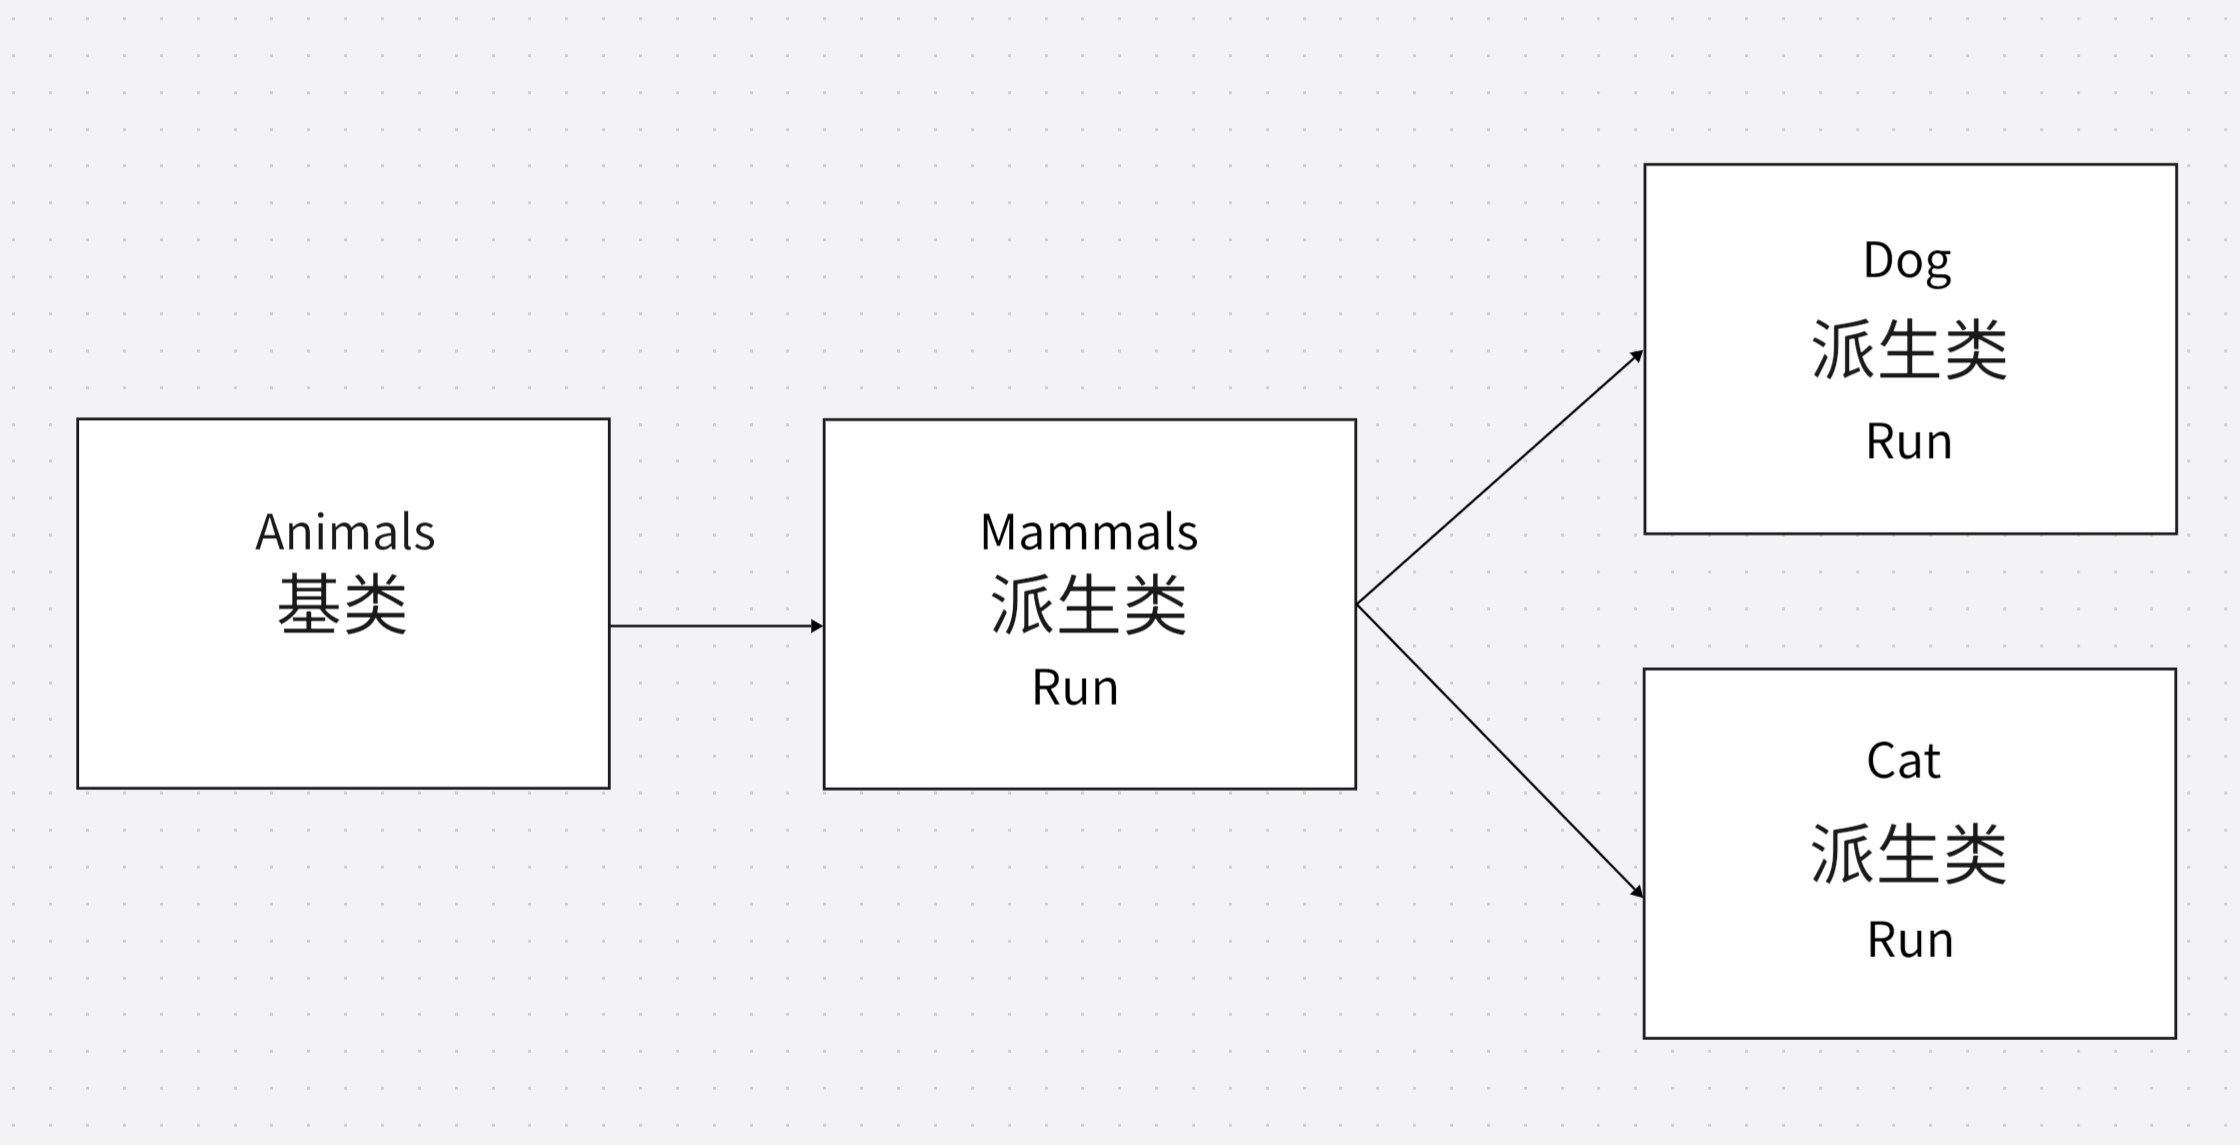
\includegraphics[width=0.7\textwidth]{A111.png}
    \caption{类的继承} % 图片标题
    \label{fig:A111} % 图片标签,用于引用
\end{figure}

如图\ref{fig:A111}所示,派生类从基类中继承了数据成员和成员函数,并可以添加新的成员。
派生类可以重写基类中的成员虚函数,从而实现新的功能。
派生类可以重载基类中的运算符,从而实现新的运算。

\begin{center}
\textbf{继承的三种方式:}

    \begin{tabular}{cccc}
        \hline
        访问 & public & private & protected \\
        \hline
        同一个类 & yes & yes & yes \\
        派生类 & yes & no & yes \\
        类外部 & yes & no & no \\ 
        \hline
        
    \end{tabular}
\end{center}

继承可以用下面的写法实现:

\begin{tcode}
class Shape {//这个基类只含有纯虚函数,又叫做抽象类
public:
    Shape() = delete;
    Shape(double A):Area(A)
    {std::cout << "基类的构造函数已经被调用" << std::endl;}
    virtual double calArea() = 0; //这里是纯虚函数,也可以使用普通函数
    double Area;
};

class Rectangle
        : protected Shape{
public:
    Rectangle() = delete;
    Rectangle(double a,double b):a(a),b(b),Shape(a*b)
    {std::cout << "Rectangle类的构造函数已经被调用,面积为" << Area << std::endl;}
    double a;
    double b;
    double calArea() override{  //重写基类的函数
        return a*b;
    }

};

class Circle
        :Shape{
public:
    Circle() = delete;
    explicit Circle(double r):r(r),Shape(3.14*r*r)
    {std::cout << "Circle类的构造函数已经被调用,面积:" << Area << std::endl;}
    double r;
    double calArea() override{
        return 3.14*r*r;
    }

};

int main(int argc, char *argv[]) {
    Circle circle(1.0);
    Rectangle rect(1.0,2.0);
    return 0;
}
\end{tcode}


 \subsubsection{模版}
在开发过程中,我们可能会遇到这样的场景,我们有一个函数或者类,但是它只适用于特定的数据类型,
比如$int$或者$double$。为了实现对这两种类型都可以调用函数,
就会遇到需要复制一遍代码,但是这样做就造成了代码冗余,不利于维护。这时候就需要用到模版($template$)。

模版是C++中一个重要的特性,它允许我们定义一个类或函数,使其可以接受不同的数据类型或者不同的参数。
模版的定义和使用都比较复杂,这里只介绍最基本的用法。
使用$class$关键字声明类型,使用具体的类型声明参数
\textbf{函数模版}的语法如下:
\begin{tcode}
template<class T>
T function(T a){
    return a;
}

auto funcPtr = function<int>;
template<int A>
int function(){
 return A;
}

auto funcPtr = function<2>;
template<class T,T A>
T function(){
 return A;
}
auto funcPtr = function<int,2>;
\end{tcode}

 这里的$class \quad T$表示一种数据类型,可以是任意类型。
 在函数的定义中,$T$可以作为函数的参数,也可以作为函数的局部变量。在使用函数模板时,需要首先进行函数的实例化。

\begin{tcode}
//调用的时候实际上分为两步,实例化和调用
function<int>(10);
function<double>(20.0);
//在编译器可以推导出类型的时候可以不加<>
auto a = function(1.0);
//在无法推导的时候,要先进行实例化
std::function<int(int)> ptr = function<int>;
\end{tcode}

模版的优点:
\begin{enumerate}
    \item 代码重用性高:可以定义一个通用的函数,然后根据需要实例化不同的类型,实现代码的重用。
    \item 类型安全:模版可以保证类型安全,避免类型错误。
    \item 效率高:模版可以提高效率,因为编译器可以对代码进行优化。
\end{enumerate}

\textbf{类模版}:
类模板的语法和函数模板类似,只不过在类名而不是函数名前面加上关键字$template$。
在普通类中也可以添加成员函数模版,只需要在函数名前面加上关键字$template$即可。

\begin{tcode}
template<class T1,class T2>
class A{
    A() = default;
    ~A() =default;
    T1 val;
    T2 id;
    T1 function(T1* a, T2& b){
        return *a+b++;
    }
};
\end{tcode}

在$template$后面,可以定义多个类型参数,用逗号分隔。需要注意的是,在类中的函数模版需要再头文件中实现,
也就是说,模版的声明和实现不可以分离,否则会出现很多问题。
对于类模板也可以实现继承和多态,与普通类相同,这里不在展开,感兴趣的同学可以自行探索。

\textbf{模板的实例化}:
模板的实例化指的是将模板定义和具体的类型绑定在一起,生成一个具体的类或函数。
在类的实例化时,$<>$的内部需要填写一个可以推导出的数据类型,编译器会根据类型推导出模板的具体类型。
一般来说,实例化有以下几种方式:

\begin{enumerate}
    \item 具体类型:如$int$,$double$等基本类型,$struct$,$class$,$union$等复合数据类型,$int*$,$double\&$等指针和引用类型
    \item 编译期可以确定的常数:字面常量,宏,$constexpr$
    \item 显示实例化:在编译时,通过命令行指定具体的类型
\end{enumerate}

除此之外,还有一种变参模版,它可以接受任意数量的类型参数,但是在实例化时,必须指定具体的类型。
这种情况比较复杂,这里不在展开。感兴趣的同学自行探讨:

\url{https://blog.csdn.net/fl2011sx/article/details/128077440}
